\documentclass[12pt]{article} % Document class
% Packages
\usepackage[utf8]{inputenc} % Input encoding (UTF-8 recommended)
\usepackage[T1]{fontenc}    % Font encoding
\usepackage{lipsum}         % Lorem Ipsum dummy text
\usepackage{graphicx}       % For including images
\usepackage{float}          % For precise figure placement
\usepackage{tabularray}     % For creating tables
\usepackage{hyperref}       % For hyperlinks

\usepackage{indentfirst}    %To indent ever paragraph

\usepackage[margin=1in]{geometry} %Chnages margin

\usepackage{fancyhdr}

\pagestyle{fancy}
\fancyhf{} % Clear the header and footer

\lhead{\projectTitle}
\rhead{\reportTitle}


\fancyfoot[R]{\latestVersion}
\fancyfoot[C]{\thepage}

\newcommand*{\nsection}[1]{
    \section*{#1}
    \addcontentsline{toc}{section}{#1}
}

\usepackage{listings}

\usepackage{xcolor}

\definecolor{codegreen}{rgb}{0,0.6,0}
\definecolor{codegray}{rgb}{0.5,0.5,0.5}
\definecolor{codepurple}{rgb}{0.58,0,0.82}
\definecolor{backcolour}{rgb}{0.95,0.95,0.92}

\lstdefinestyle{mystyle}{
    backgroundcolor=\color{backcolour},   
    commentstyle=\color{codegreen},
    keywordstyle=\color{magenta},
    numberstyle=\tiny\color{codegray},
    stringstyle=\color{codepurple},
    basicstyle=\ttfamily\footnotesize,
    breakatwhitespace=false,         
    breaklines=true,                 
    captionpos=b,                    
    keepspaces=true,                 
    numbers=left,                    
    numbersep=5pt,                  
    showspaces=false,                
    showstringspaces=false,
    showtabs=false,                  
    tabsize=2
}

\lstset{style=mystyle}



\newcommand{\projectTitle}{Git Guide}
\newcommand{\reportTitle}{How to Git}
\newcommand{\latestVersion}{Version 0.0.1}


\begin{document}

\titleformat{name =\section, numberless}[display] {\huge\bfseries}{}{0pt}{\fontsize{22}{28}\selectfont\addcontentsline{toc}{section}}

% Create the title page

\clearpage
\pagenumbering{roman}
\setcounter{page}{1}

\begin{figure}
	\centering
	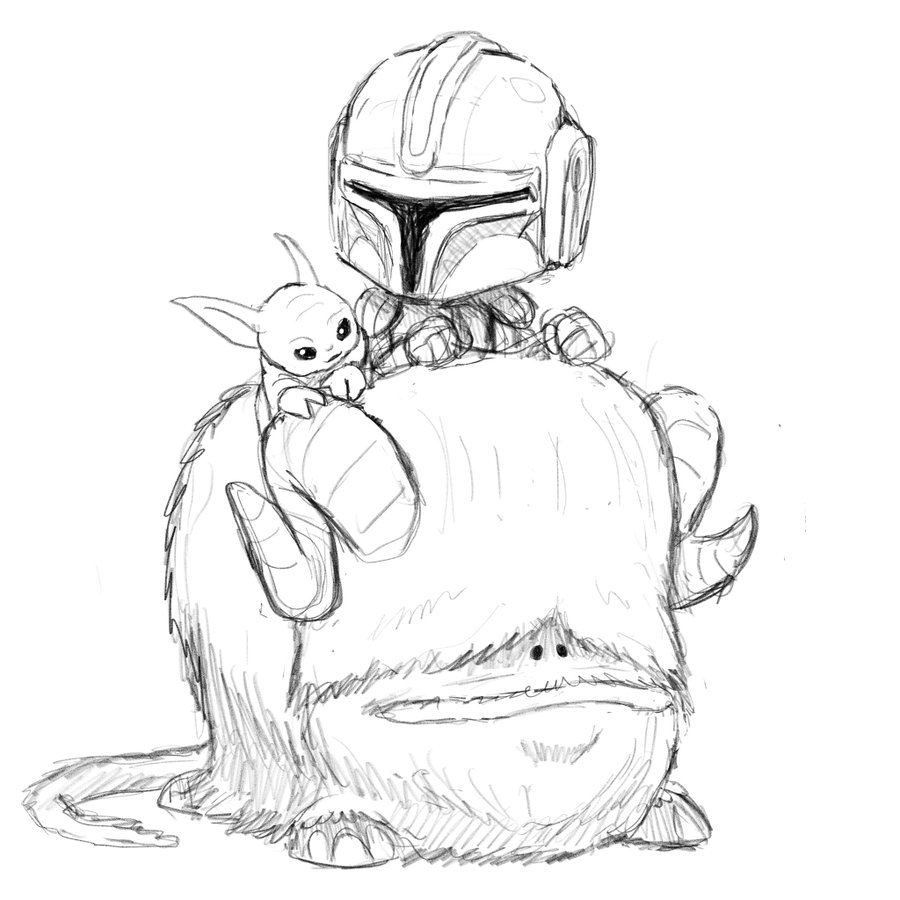
\includegraphics[width=3cm]{Fun_pics/bantha_inc.jpg}
\end{figure}

\begin{center}
	\textbf{\LARGE Bantha Inc.} \\
	\vspace{1cm}
	\Large \today \\
	\vspace{0.3cm}

	\rule{\linewidth}{0.5pt} \\
	\vspace{0.2cm}
\LARGE \projectTitle \\ \vspace{0.3cm} \large \reportTitle\\


	\vspace{0.1cm}
	\rule{\linewidth}{0.5pt} \\

	\vspace{1.5cm}

	\begin{tabular}{lr}
		\textit{Author:} & Die Go \\
	\end{tabular}

	\vspace{1cm}
	\date{}
\end{center}


\newpage
\section{Revision History} % Section 1
\begin{center}
    \begin{tblr}{
        hlines,
        vlines,
        %row{1} = {bg=gray,fg=white},
        %row{2} = {bg=green9},
        rows = {ht=.55cm, valign=m},
        columns = {halign=c},
        %colspec = {Q[1cm,bg=gray,fg=white] XXX},} 
        %colspec = {Q[2cm] XXX},} 
        colspec = {Q[3cm] XXX},} 
        \textbf{Date} & \textbf{Version} & \textbf{Author} & \textbf{Description} \\
        08SEP2023 & 0.0.1 & Diego F. & Template Created \\
        09SEP2023 & 0.0.2 & Diego F. & Executive Summary \\
    \end{tblr}
\end{center}

% Table of Contents
\newpage
\tableofcontents

% List of Figures
\newpage
\listoffigures

% List of Tables
\newpage
\listoftables

%Start of report
\newpage
\pagenumbering{arabic}
\setcounter{page}{1}


\section{Introduction}
This is a guide of how to do Git. It is a really beginner thing as I will go through from how start a repo to some really cool stuff. I try to explain what stuffs does. 

\section*{Methods} % Section 3
% ... (unchanged content)

\section{Results} % Section 4
% ... (unchanged content)

\subsection{Figures} % Subsection 4.1
% ... (unchanged content)

\section{Conclusion} % Section 5
% ... (unchanged content)

\subsection{Tables} % Subsection 5.1
% ... (unchanged content)

\end{document}
